\chapter{Aggiunta dei filtri di Bloom a Redis}

\section{Obiettivo}

L'obiettivo della modifica a Redis svolta per questa tesi è introdurre il supporto per i filtri di
Bloom. È stato effettuata prima una fase di progettazione dei nuovi comandi da aggiungere e di
conseguenza della variante esatta di filtro da implementare; è stata preparata una prima
implementazione completa di copertura tramite test automatizzati; infine, sono state effettuate
delle analisi sui parametri di configurazione di default, cercando di studiare il compromesso tra
utilizzo della memoria, tempo di esecuzione, e probabilità di falsi positivi.

\section{Scelta della variante di filtro}

Nella fase iniziale di design, abbiamo comunicato più volte con l'autore di Redis (Salvatore
Sanfilippo), cercando di stabilire insieme i requisiti che l'implementazione del filtro dovesse
avere perché la modifica corrispondesse agli standard di Redis.

In particolare, abbiamo identificato i seguenti requisiti:

\begin{itemize}
	\medskip
	\item \textbf{Dinamicità}: tutte le strutture dati di Redis sono dinamiche, cioè è possibile
	aggiungere elementi illimitati, con l'unico vincolo rappresentato dalla memoria a disposizione
	sul sistema. Nessuna struttura dati richiede un dimensionamento fisso.

	\item \textbf{Scalabilità}: l'utilizzo della memoria deve essere molto contenuto quando la
	struttura dati contiene pochi elementi, e crescere gradualmente all'aumentare degli elementi.
	Eventuali pre-allocazioni devono essere molto limitate. Per esempio, non sarebbe accettabile che
	il filtro possa occupare \SI{1}{\mega\byte} di RAM alla creazione.

	\item \textbf{Scarsa configurabilità}: Redis cerca di offrire strutture dati che siano
	preconfigurate con default accettabili per la maggior parte dei casi d'uso, e offre la minima
	configurabilità necessaria ad operare negli scenari applicativi previsti. In particolare,
	i filtri di Bloom hanno diversi parametri a disposizione e sono quindi richieste scelte
	oculate.
\end{itemize}

Per soddisfare i requisiti, ci si è orientati su implementare i filtri di Bloom scalabili
(\autoref{sec:bloomscalable}), i quali eliminano la necessità di determinare in anticipo il
dimensionamento della struttura (in termini di byte o di numero di elementi), e la cui crescita
esponenziale di occupazione della memoria consente una sostanziale scalabilità.

Si è ritenuto essenziale esporre all'applicativo che utilizza Redis il parametro $P$ di probabilità
di falso positivo, poiché strettamente legato al tipo di scenario e al bilanciamento richiesto di
performance e uso della memoria, nascondendo quindi all'utente tutti i parametri più tecnici
(fattore di intensificazione $r$, fattore di crescita $s$, tipologia di funzione di hash), che
rimangono quindi fissati al momento della compilazione di Redis. Nonostante questo, anche per il
parametro $P$ ci si è orientati su offrire un default, rendendo più semplice per l'utente iniziare
l'utilizzo della struttura dati, anche in fase di sviluppo.

\section{Progettazione dei nuovi comandi}
\label{sec:patch:newcommands}

Nel progettare i nuovi comandi, abbiamo cercato di adeguarci il più possibile allo stile dei
comandi esistenti, cercando di mantenere le proprietà evinte durante la fase di analisi.

Abbiamo scelto il prefisso~\cverb|BF| per la famiglia di comandi, indicando chiaramente la
struttura dati che viene manipolata.

Questi sono i comandi implementati:

\begin{description}[style=nextline,font={\bfseries\ttfamily}]
	\item[{BFADD key [ERROR p] ELEMENTS ele [ele2\dots]}] Aggiunge uno o più elementi al
	filtro di Bloom specificato, creandolo se non già esistente. Restituisce il numero degli
	elementi che risultavano non presenti al momento dell'inserimento (dato soggetto quindi ad
	errore).

	L'errore $P$ può essere indicato opzionalmente solo al momento della creazione, cioè del primo
	inserimento; se viene specificato in un filtro già esistente, e il valore specificato è diverso
	da quello con cui il filtro è stato creato, il comando restituisce un errore senza effettuare
	alcun inserimento.

	\item[BFEXIST key ele] Verifica la presenza di un elemento nel filtro specificato
	(test di appartenenza). Se il filtro non esiste, il comando restituisce falso.

	\item[BFCOUNT key] Restituisce una stima del numero di elementi inseriti nel filtro.
	Se il filtro non esiste, il comando restituisce $0$.

	\item[BFDEBUG] Restituisce informazioni utili al debugging dell'implementazione del
	filtro. Questo comando accetta come primo parametro un sotto-comando; al momento, ne sono stati
	implementati due:

		\begin{description}[style=nextline,font={\bfseries\ttfamily}]
		\item[BFDEBUG STATUS key] Restituisce una stringa che contiene informazioni sullo
		stato attuale del filtro, e in particolare il numero di filtri presenti nella catena, e
		l'errore che è stato specificato.

		\item[BFDEBUG FILTER key idx] Restituisce informazioni su uno specifico filtro
		della catena; il filtro che si vuole ispezionare deve essere specificato come indice 
		nel parametro \cverb|idx|. La stringa restituita mostra il numero di sezioni (o funzioni
		di hash), la dimensione in bit di una sezione e il numero di bit impostati a 1.
		\end{description}

\end{description}

Si noti come, avendo esposto il solo parametro di probabilità, di fatto i comandi si applicano ad
una qualunque struttura dati probabilistica che implementa un insieme, consentendo in futuro di
cambiare implementazione se lo si ritenesse necessario, senza invalidare l'utilizzo da parte dei
client. I comandi di Redis, infatti, mantengono una compatibilità completa rispetto alla prima
versione in cui vengono implementati, in modo che sia sempre possibile aggiornare il server senza
causare problemi ai client.

\section{Esempio d'uso dei comandi}

Vediamo ora un esempio di sessione utilizzando i comandi appena descritti:

\medskip
\begin{commentedsource}[style=redis,caption=Esempio di utilizzo dei nuovi comandi per i filtri di Bloom]
|\lnote|127.0.0.1:6379> BFADD prova ELEMENTS a b c d e
(integer) 5
|\lnote|127.0.0.1:6379> BFCOUNT prova
(integer) 5
|\lnote|127.0.0.1:6379> BFADD prova ELEMENTS f g a
(integer) 2
127.0.0.1:6379> BFCOUNT prova
(integer) 7
|\lnote|127.0.0.1:6379> BFEXIST prova b
(integer) 1
127.0.0.1:6379> BFEXIST prova z
(integer) 0
|\lnote|127.0.0.1:6379> BFDEBUG STATUS prova
"n:1 e:0.003"
|\lnote|127.0.0.1:6379> BFDEBUG FILTER prova 0
"k:12 s:1811 b:84"
\end{commentedsource}

Per cominciare, viene creato un filtro chiamato \cverb|prova| \lnnum{1} in cui vengono inseriti 5
elementi (ciascun elemento è una stringa di un solo carattere, corrispondenti alle prime cinque
lettere dell'alfabeto). Il comando restituisce il valore $5$, corrispondente al numero di elementi
inseriti. Viene poi effettuato un calcolo della cardinalità stimata \lnnum{2}, che
restituisce il valore corretto $5$.

Successivamente, viene fatto un secondo inserimento \lnnum{3}; questa volta, oltre a due
elementi nuovi (stringhe \cverb|f| e \cverb|g|), viene inserito anche un elemento che era stato
già precedentemente inserito: la lettera \cverb|a|. Il comando restituisce $2$, riportando
correttamente il numero di nuovi elementi inseriti, e anche il successivo calcolo della
cardinalità è corretto, poiché restituisce $7$.

Poi viene effettuato un primo test di appartenenza al filtro tramite il comando \cverb|BFEXIST|
\lnnum{4}, richiedendo se l'elemento corrispondente alla stringa \cverb|b| è presente; l'elemento era
stato inserito precedentemente \lnnum{1}, ed infatti il comando restituisce correttamente $1$ per
indicare che l'elemento è presente. Successivamente, viene effettuato un secondo test con l'elemento
\cverb|z| che non era stato mai inserito, e il comando questa volta restituisce $0$.

Il comando \cverb|BFDEBUG STATUS| viene usato per ispezionare lo
stato del filtro \lnnum{5}. La stringa restituita è composta da due valori:

\medskip
\begin{tabular}{ |l|l|p{240pt}| }
  \hline
  $n$ & $1$ & La catena del filtro scalabile contiene un solo filtro \\
  $e$ & $0.003$ & La probabilità di falsi positivi è impostata a \SI{0.3}{\percent} \\
  \hline
\end{tabular}
\medskip

Per finire, il comando \cverb|BFDEBUG FILTER| serve a ispezionare lo stato del primo filtro della
catena \lnnum{6}. La stringa restituita contiene tre valori:

\medskip
\begin{tabular}{ |l|l|p{240pt}| }
  \hline
  $k$ & $11$ & Il filtro utilizza $11$ funzioni di hash, cioè è diviso in $11$ sezioni \\
  $s$ & $1798$ & Ciascuna sezione è formata da \SI{1798}{\bit}, per un totale di $\num{1798 x 11} =
  \SI{19778}{\bit}$ \\
  $b$ & $77$ & Al momento ci sono \SI{77}{\bit} impostati a $1$. Questo corrisponde infatti a $7$
  elementi inseriti con $11$ funzioni di hash, e senza che si sia verificata alcuna collisione. \\
  \hline
\end{tabular}
\medskip

Per modificare la probabilità di falso positivo di un filtro, è possibile specificare un valore
durante il primo inserimento:

\medskip
\begin{commentedsource}[style=redis,caption=Filtro con probabilità configurata dall'utente]
|\lnote|127.0.0.1:6379> BFADD esempio ERROR 0.05 ELEMENTS a b c d e f g
(integer) 7
127.0.0.1:6379> BFDEBUG STATUS esempio
"n:1 e:0.05"
127.0.0.1:6379> BFDEBUG FILTER esempio 0
|\lnote|"k:8 s:3344 b:56"
\end{commentedsource}

In questo caso il filtro viene creato con una probabilità di falso positivo del \SI{5}{\%},
specificata tramite il parametro \cverb|ERROR 0.05| \lnnum{1}. Vengono poi inseriti i medesimi
elementi dell'esempio precedente, ed è possibile verificare che i parametri del primo filtro 
della catena sono ora diversi \lnnum{2}: in particolare, sono sufficienti $8$ funzioni di hash
contro le $12$ usate precedentemente; il numero di bit impostati è quindi anch'esso inferiore
($56$), portando quindi ad un uso minore di memoria a parità di elementi, come ci si aspetta
aumentando l'errore consentito.

\section{Analisi delle modifiche effettuate}
\label{sec:patchexplain}

Le modifiche effettuate a Redis sono disponibili su GitHub, all'interno del
\fnhref{https://github.com/rasky/redis/tree/bloomfilter}{repositorio fork di Redis}, in un branch
chiamato \cverb|bloomfilter|, e la parte principale del codice è riportata anche
nella \autoref{sec:modredis}.

\subsection{Strutture dati}

Nel file \cverb|bloom.h| vengono definite le due strutture dati principali:

\begin{commentedsource}[style=csource,caption=Strutture dati,label={lst:bloomStruct}]
typedef struct filter {
    struct filter *next;  /* next filter in chain */
    uint64_t s;           /* size of each partition in bits */
    uint64_t b;           /* number of bits set in this filter */
    uint64_t bmax;        /* maximum number of bits that should be set */
    uint32_t k;           /* number of partitions */
    uint8_t *parts[];
} filter;

typedef struct bloom {
	double e;             /* requested false positive probability */
	int numfilters;       /* number of filters in the chain */
	filter *first;        /* first filter in the chain */
} bloom;
\end{commentedsource}

La struttura \cverb|bloom| rappresenta l'intero filtro scalabile. I suoi campi sono
così definiti:

\medskip
\begin{tabular}{ |l|l|p{200pt}| }
  \hline
  \cverb|e| & \cverb|double| & La probabilità richiesta di un falso positivo. Questo è il valore richiesto
  dall'utente, che il filtro cercherà di rispettare come margine superiore. \\

  \cverb|numfilters| & \cverb|int| & Numero di filtri presenti nella catena. \\

  \cverb|first| & \cverb|filter*| & Puntatore alla testa della lista concatenata di filtri. \\
  \hline
\end{tabular}
\medskip

Come si evince, i filtri sono conservati in una lista a catena singola, e il campo \cverb|first|
contiene il puntatore alla testa. La scelta di una lista per l'implementazione della catena di
filtri semplifica l'implementazione ed è compatibile con gli algoritmi che la utilizzano poiché
molto spesso è richiesto di attraversare l'intera catena, mentre per esempio l'accesso casuale non è
mai richiesto.

Ciascun filtro è rappresentato dalla struttura \cverb|filter|, definita dai seguenti campi:

\medskip
\begin{tabular}{ |l|l|p{210pt}| }
  \hline

  \cverb|next| & \cverb|filter*| & Puntatore al filtro successivo nella catena \\

  \cverb|k| & \cverb|uint32| & Numero di funzioni di hash (e dunque di partizioni) \\

  \cverb|b| & \cverb|uint64| & Numero di bit attualmente impostati a $1$, considerando tutte le partizioni \\

  \cverb|s| & \cverb|uint64| & Dimensione di ciascuna partizione in bit. L'utilizzo di memoria
  effettivo è $\ceil{s/7}$ \\

  \cverb|bmax| & \cverb|uint64| & Numero di bit che possono essere impostati al massimo a $1$ prima
  che venga raggiunta la densità scelta come obiettivo (tipicamente, \SI{50}{\percent}). \\

  \cverb|parts| & \cverb|uint8*[]| & Array di puntatori alle partizioni. \\

  \hline
\end{tabular}
\medskip

Si noti che l'array \cverb|parts| è definito a dimensione variabile (anche detto \emph{array
flessibile}), utilizzando la funzionalità introdotta nello standard C99 che consente all'ultimo
membro di una struttura, se array, di avere una dimensione non dichiarata staticamente, ma gestita
dinamicamente al momento di allocare la struttura stessa sullo heap. Poiché la dimensione dell'array
è pari a \cverb|k| e non cambia mai dopo l'inizializzazione della struttura, questa scelta consente
di allocare la struttura \cverb|filter| e l'array di puntatori dinamico con una sola allocazione.

\subsection{Parametri di configurazione statici}
\label{sec:patch:staticparms}

All'inizio del file \cverb|bloom.c|, troviamo alcune costanti di configurazione per le quali si è
preferito non esporre una configurazione a livello utente.

\begin{commentedsource}[style=csource,caption=Parametri statici]
/* Initial desired size of the bloom filter (in bytes). */
#define CONFIG_BLOOM_BASESIZE 2048 

/* Default false-positive error rate */
#define CONFIG_BLOOM_DEFAULTERROR 0.003

/* Fill ratio of a filter before it is considered full. We also call this P */
#define CONFIG_BLOOM_DESIREDFILLRATIO 0.5

/* Desired growth for items, for each new allocated filter.
 * Default is 2.0, which means that each new filter should hold
 * twice as many items as the previous one. */
#define CONFIG_BLOOM_ITEMGROWTHRATIO 2.0

/* Desired tightening ratio for false-positive error.
 * Each new filter must have a tighten error ratio compared to
 * the previous one, to asymptotically approach the user-requested
 * ratio. */
#define CONFIG_BLOOM_TIGHTENINGRATIO 0.85
\end{commentedsource}

Questa la descrizione dettagliata di ciascun parametro:

\medskip
\begin{itemize}
  \item \cverb|CONFIG_BLOOM_BASESIZE| (\SI{2048}{\byte}). Dimensione iniziale in byte del primo
  filtro della catena. La dimensione è stata calcolata tenendo conto di un bilanciamento tra uso
  della memoria, crescita del numero di filtri nella catena, e velocità (vedi la
  \autoref{sec:patch:basesize}).

  \item \cverb|CONFIG_BLOOM_DEFAULTERROR| ($\SI{0.3}{\percent}$). Probabilità di default di falso
  positivo a cui il filtro scalabile tende asintoticamente. La scelta del valore cerca di
  massimizzare i casi d'uso in cui il filtro può essere usato con successo (vedi la
  \autoref{sec:patch:defaulterror}).

  \item \cverb|CONFIG_BLOOM_DESIREDFILLRATIO| ($\SI{50}{\percent}$). Valore di densità massimo dei filtri
  nella catena; quando il filtro in fondo alla catena (l'unico su cui si inseriscono nuovi elementi)
  raggiunge questa densità, un nuovo filtro viene creato. Il valore ottimizza l'uso dei filtri di
  Bloom, come visto nella \autoref{sec:bloomparms}.

  \item \cverb|CONFIG_BLOOM_ITEMGROWTHRATIO| ($\num{2.0}$). Fattore di crescita dei filtri
  all'interno della catena. Come visto nella \autoref{sec:bloomscalable} dove è chiamato
  $s$, questo fattore delinea una progressione geometrica che consente di adattare la crescita del
  filtro all'aumentare del numero di elementi inseriti senza creare una catena troppo lunga
  né sprecando troppa memoria.

  \item \cverb|CONFIG_BLOOM_TIGHTENINGRATIO| ($\num{0.85}$). Fattore di intensificazione, applicato
  per creare una progressione geometrica tra le probabilità di falsi positivi dei filtri all'interno
  della catena, come descritto nella \autoref{sec:bloomscalable}. Il valore ottimale è indicato
  essere compreso in $\interval{0.8}{0.9}$ in \cite{bloom-scalable}.

\end{itemize}
\medskip

\subsection{Creazione e distruzione di un filtro}

La creazione e distruzione di un intero filtro scalabile è implementata dalle seguenti funzioni:

\begin{commentedsource}[style=csource,caption=Creazione e distruzione di un filtro scalabile]
bloom *bloomNew(void) {
/*@\lnote@*/	bloom *bf = zmalloc(sizeof(bloom));
	bf->numfilters = 0; 
    bf->e = CONFIG_BLOOM_DEFAULTERROR;
/*@\lnote@*/    bf->first = NULL; /* do not create filter here, because user might change error */ 
	return bf;
}

void bloomRelease(bloom *bf) {
    filter *flt = bf->first;
/*@\lnote@*/    while (flt) { 
        filter *next = flt->next;
/*@\lnote@*/        bloomFilterRelease(flt); 
        flt = next;
    }
/*@\lnote@*/    zfree(bf); 
}
\end{commentedsource}

La funzione \cverb|bloomNew| alloca una struttura di tipo \cverb|bloom| sullo heap \lnnum{1},
utilizzando la funzione \cverb|zmalloc|, una funzione interna di Redis che implementa un sottile
strato di codice sopra l'allocatore standard per tracciare l'occupazione totale di memoria e fornire
informazioni utili a livello statistico e per debugging.

Si noti che durante la creazione del filtro scalabile, la catena viene lasciata completamente vuota
\lnnum{2}: ritardando la creazione del primo filtro della catena all'inserimento del primo elemento,
è possibile infatti accorgersi velocemente se, in un dato momento, è stato mai inserito un elemento,
caratteristica utile alla corretta implementazione del comando \cverb|BFADD| che deve discriminare il
primo inserimento per permettere la configurazione del parametro di errore.

La funzione \cverb|bloomRelease| rilascia la memoria allocata dall'intero filtro scalabile,
percorrendo la catena \lnnum{3} e chiamando la funzione di distruzione di ciascun filtro \lnnum{4},
terminando poi rilasciando la memoria occupata dalla struttura del filtro stessa \lnnum{5}.

\begin{commentedsource}[style=csource,caption=Creazione e distruzione di un filtro,label={lst:bloomFilterNew}]
filter* bloomFilterNew(bloom *bf) {
    int idx = bf->numfilters;

    /* Compute N0 (N for the first filter) so that the first M (memory size)
     * will match BLOOM_BASE_SIZE. */
    uint32_t n0 = CONFIG_BLOOM_BASESIZE*8 * ((log(CONFIG_BLOOM_DESIREDFILLRATIO) * log(1-CONFIG_BLOOM_DESIREDFILLRATIO)) / fabs(log(bf->e)));

    /* Compute E0 (E for the first filter) so that the composed probability converges to E. */
/*@\lnote@*/    double e0 = bf->e * (1 - CONFIG_BLOOM_TIGHTENINGRATIO);

    /* Compute input parameters for the new filter, iterating exponentially
     * given the configured ratios. */
    uint32_t n = n0 * pow(CONFIG_BLOOM_ITEMGROWTHRATIO, idx);
    double e = e0 * pow(CONFIG_BLOOM_TIGHTENINGRATIO, idx);

    /* Compute derived parameters */
/*@\lnote@*/    int k = ceil(-log2(e));
/*@\lnote@*/    uint64_t m = (double)n / ((log(CONFIG_BLOOM_DESIREDFILLRATIO) * log(1-CONFIG_BLOOM_DESIREDFILLRATIO)) / fabs(log(e)));
    uint64_t s = m / k;
    uint64_t bmax = (s*k) * CONFIG_BLOOM_DESIREDFILLRATIO;

/*@\lnote@*/    filter *flt = zmalloc(sizeof(filter) + k*sizeof(void*));
    flt->next = NULL;
    flt->s = s;
    flt->k = k;
    flt->b = 0;
    flt->bmax = bmax;
/*@\lnote@*/    for (int i=0;i<k;i++) {
        uint32_t bsize = (flt->s + 7) / 8;
        flt->parts[i] = zmalloc(bsize);
        memset(flt->parts[i],0,bsize);
    }
    bf->numfilters++;
    return flt;
}

void bloomFilterRelease(filter *flt) {
/*@\lnote@*/    for (unsigned int i=0;i<flt->k;i++)
        zfree(flt->parts[i]);
/*@\lnote@*/    zfree(flt);
}
\end{commentedsource}

La funzione \cverb|bloomFilterNew| riceve in input un filtro scalabile e ritorna un filtro appena
creato con i parametri adatti ad essere l'ultimo filtro della catena.

Il calcolo dei parametri del filtro ricalca quanto visto nella \autoref{sec:bloomparms} e nella
\autoref{sec:bloomscalable}. In particolare, \lnnum{1} segue la \autoref{eq:p0fromp}, \lnnum{2} 
segue la \autoref{eq:bloomk}, e \lnnum{3} segue la \autoref{eq:bloomm}.

Si può notare come la memoria allocata tenga conto dell'array flessibile delle sezioni, lasciando lo
spazio per il giusto numero di puntatori (uno per sezione) \lnnum{4}. Nel ciclo successivo
\lnnum{5}, vengono allocate invece le singole sezioni ed inizializzate a $0$.

La cancellazione di un filtro avviene tramite una chiamata alla funzione \cverb|bloomFilterRelease|,
che semplicemente rilascia la memoria di tutte le sezioni \lnnum{6}, e infine la memoria del filtro
stesso \lnnum{7}.

\subsection{Aggiunta di un elemento al filtro}

Vediamo ora come viene aggiunto un elemento ad un filtro. Una prima funzione \cverb|bloomAdd| si
occupa di individuare il filtro giusto all'interno della catena:

\begin{commentedsource}[style=csource,caption=Aggiunta elemento ad un filtro scalabile]
int bloomAdd(bloom *bf, unsigned char *ele, size_t elesize) {
    /* Go to the last filter, which is the current one */
    filter *flt = bf->first;
    if (!flt)
/*@\lnote@*/        flt = bf->first = bloomFilterNew(bf);
    else {
/*@\lnote@*/        while (flt->next)
            flt = flt->next;

        /* Check if this bloom filter is full; if so, allocate
         * a new one */
        if (flt->b >= flt->bmax) {
/*@\lnote@*/            flt->next = bloomFilterNew(bf);
            flt = flt->next;
        }
    }

    /* Add the element to the filter */
/*@\lnote@*/    return bloomFilterAdd(flt, ele, elesize);
}
\end{commentedsource}

L'obiettivo della funzione è identificare il filtro corrente nella catena, cioè l'unico dentro cui è
possibile aggiungere elementi (poiché tutti gli altri avranno già raggiunto la densità massima), per
poi aggiungervi l'elemento tramite la funzione \cverb|bloomFilterAdd| \lnnum{4}.

Se la catena è vuota, viene immediatamente creato il primo filtro \lnnum{1}, che diventa il
corrente. Altrimenti, si percorre la catena fino ad arrivare all'ultimo filtro \lnnum{2}; se anche
esso ha superato la densità massima configurata, viene aggiunto un nuovo filtro vuoto in fondo alla
catena, usando \cverb|bloomFilterNew| \lnnum{3}: questo è il momento in cui il filtro scalabile
cresce.

Vediamo ora il dettaglio dell'aggiunta dell'elemento ad un singolo filtro.

\begin{commentedsource}[style=csource,caption=Aggiunta elemento ad un filtro,label={lst:bloomFilterAdd}]
uint64_t bloomFilterHash(unsigned char *ele, size_t elesize) {
/*@\lnote@*/    return MurmurHash64A(ele,elesize,0xc5fb9af2ULL);
}

int bloomFilterAdd(filter *flt, unsigned char *ele, size_t elesize) {
    /* Calculate initial hash for the element. Since 32-bit index is enough,
       we use a 64-bit hash as two 32-bit hashes. */
    uint64_t hash = bloomFilterHash(ele,elesize);
/*@\lnote@*/    uint32_t a = (uint32_t)hash;
    uint32_t b = (uint32_t)(hash>>32);
    int nbits = 0;

    for (unsigned int i=0;i<flt->k;i++) {
        /* To compute multiple hash functions from two hashes,
         * we use the algorithm described here:
         * http://www.eecs.harvard.edu/~michaelm/postscripts/rsa2008.pdf
         */
/*@\lnote@*/        uint64_t index = a;
        a += b; b += i; 

        /* Use fast unbiased modulo reduction, instead of "% size".
         * See http://lemire.me/blog/2016/06/27/a-fast-alternative-to-the-modulo-reduction/ */
/*@\lnote@*/        index = (index * flt->s) >> 32;

        /* Turn on the correct bit in each partition */
/*@\lnote@*/        nbits += (flt->parts[i][index>>3] & (1 << (index&7))) ? 0 : 1;
/*@\lnote@*/        flt->parts[i][index>>3] |= 1 << (index&7);
    }

    /* Keep count of total bits set to 1 */
/*@\lnote@*/    flt->b += nbits;

    /* If at least one bit was turned off, we consider the item really added. */
    return nbits > 0;
}
\end{commentedsource}

La funzione \cverb|bloomFilterAdd| effettua invece l'inserimento vero e proprio, secondo
l'\autoref{alg:bloominsert} visto nella \autoref{sec:bloom:add}.

Per le funzioni di hash, viene utilizzato l'\autoref{alg:ehndoublehash} di doppio hash
avanzato, visto nella \autoref{sec:bloom:hash}. L'algoritmo richiede in partenza due funzioni di
hash ($h_a$ e $h_b$): nell'implementazione viene utilizzata la funzione di hash
\cverb|MurmurHash64A| \lnnum{1}, una variante a \SI{64}{\bit} della funzione MurMurHash2
(\autoref{alg:murmurhash2}). Di questa funzione, è presente già un'implementazione dentro il
codice sorgente di Redis, e poiché l'output è a \SI{64}{\bit}, consideriamo la suddivisione in due
valori a \SI{32}{\bit} come l'output di due funzioni di hash separate, ottenendo così i due valori
\cverb|a| e \cverb|b| \lnnum{2} utili come input per l'algoritmo di doppio hash avanzato. La funzione
\cverb|MurMurHash64A| richiede come abbiamo visto un seme; in questo caso è necessario poter 
ricostruire sempre lo stesso hash a partire dallo stesso elemento, quindi il seme deve essere
fisso. È stato quindi calcolato in fase di sviluppo un valore casuale ed inserito nel
codice (\cverb|0xc5fb9af2|).

Il calcolo del doppio hash avviene in formato iterativo \lnnum{3}, secondo quanto visto
nell'\autoref{alg:ehndoublehash}. Successivamente, viene effettuata una riduzione dell'output della
funzione di hash all'interno del dominio scelto \lnnum{4}. Invece del classico algoritmo di
riduzione $idx = hash \bmod s$ (con $s$ dimensione in bit della sezione), utilizziamo la formula
$idx = hash \times s / 2^{32}$ che effettua comunque la riduzione richiesta, considerando che $index
\in \interval[open right]{0}{2^{32}}$, ma senza richiedere una divisione, che anche nei moderni
processori ha una latenza elevata (circa $26$ cicli, contro i $4$ di una moltiplicazione). Si veda
\cite{lemire-reduction} per i dettagli relativi a questa formula di riduzione.

A questo punto, subito prima di impostare il bit a $1$, si verifica lo stato del bit \lnnum{5}; se
esso è impostato a zero, si incrementa un contatore chiamato \cverb|nbits| che tiene conto di quanti
bit hanno cambiato di stato (da zero ad uno) durante l'inserimento dell'elemento. Questo contatore,
al termine del ciclo, viene sommato al campo \cverb|b| del filtro \lnnum{7}, mantenendo così un conto
di quanti bit sono impostati a $1$ nell'intero filtro, molto utile per il calcolo della cardinalità
(vedi \autoref{sec:patch:card}).

Infine, viene impostato a $1$ il bit corrispondente all'indice \lnnum{6}, o\-pe\-ra\-zio\-ne
principale dell'algoritmo di inserimento.

\subsection{Test di appartenenza di un elemento al filtro}

Come nel precedente caso, anche per il test di appartenenza vi sono due funzioni da analizzare.
La prima, \cverb|bloomExist|, esegue un controllo sull'intera catena di filtri:

\begin{commentedsource}[style=csource,caption=Test di appartenenza di un elemento,label={lst:bloomExist}]
int bloomExist(bloom *bf, unsigned char *ele, size_t elesize) {
    /* Calculate initial hash for the element */
/*@\lnote@*/    uint64_t hash = bloomFilterHash(ele,elesize);

    /* Check all bloom filters for membership. If the element is
       found in any of them, it means it's present. */
/*@\lnote@*/    for (filter *flt = bf->first; flt; flt = flt->next)
        if (bloomFilterExist(flt,hash))
/*@\lnote@*/            return 1;
    return 0;
}
\end{commentedsource}

Utilizzando la funzione \cverb|bloomFilterHash| già vista in precedenza, viene calcolata la funzione
di hash sull'elemento del quale si vuole effettuare il test di appartenenza \lnnum{1}. Il successivo
ciclo \lnnum{2} scorre tutti i filtri della catena e richiama la funzione \cverb|bloomFilterExist|
su ciascun filtro, passando come argomento il valore di hash già calcolato. Non appena l'elemento
viene trovato all'interno di un filtro, si esce immediatamente dal ciclo restituendo un valore di
successo \lnnum{3}.

La funzione \cverb|bloomFilterExist| implementa invece il cuore del test, cioè 
l'\autoref{alg:bloomtest}:

\begin{commentedsource}[style=csource,caption=Test di appartenenza di un elemento ad un filtro]
int bloomFilterExist(filter *flt, uint64_t hash) {
/*@\lnote@*/    uint32_t a = (uint32_t)hash;
    uint32_t b = (uint32_t)(hash>>32);

    for (unsigned int i=0;i<flt->k;i++) {
        /* See bloomFilterAdd for a description of the index calculation algorithm. */
/*@\lnote@*/        uint64_t index = a;
        a += b; b += i;
        index = (index * flt->s) >> 32;

        /* For each bit, if it's not set, early exit immediately */
/*@\lnote@*/        if (~(flt->parts[i][index>>3] >> (index & 7)) & 1)
            return 0;
    }
/*@\lnote@*/    return 1;
}
\end{commentedsource}

Il calcolo dell'indice segue quanto già visto in \cverb|bloomFilterAdd|
(\autoref{lst:bloomFilterAdd}): il valore di hash a \SI{64}{\bit} viene utilizzato per estrarre due
hash a \SI{32}{\bit} \lnnum{1}, che vengono successivamente usati per il calcolo del doppio hash
secondo l'\autoref{alg:ehndoublehash} \lnnum{2}.

Una volta identificato l'indice, si verifica se il corrispondente bit è spento \lnnum{3}, nel qual
caso si restituisce immediatamente $0$ indicando così che l'elemento non è presente. Solo nel caso
in cui tutti i bit corrispondenti a tutte le funzioni di hash sono accesi, è possibile restituire il
valore $1$ \lnnum{4} che indica che il successo del test.

\subsection{Stima della cardinalità}
\label{sec:patch:card}

La stima della cardinalità viene implementata dalla funzione qui riportata, \cverb|bloomCard|:

\begin{commentedsource}[style=csource,caption=Stima della cardinalità]
int bloomCard(bloom *bf) {
    int nelem = 0;

    /* Sum cardinality estimation of each filter. */
/*@\lnote@*/    for (filter *flt = bf->first; flt; flt = flt->next) {
/*@\lnote@*/        double p = ((double)flt->b / (double)flt->bmax) * CONFIG_BLOOM_DESIREDFILLRATIO;
/*@\lnote@*/        nelem += floor((double)flt->s * -log(1.0-p) + .5);
    }
    return nelem;
}
\end{commentedsource}

Poiché un filtro scalabile è composto da una catena di filtri riempiti in sequenza, la stima
della cardinalità è data dalla somma della cardinalità stimata in ciascun filtro, secondo 
l'\autoref{eq:bloomcard}. Il ciclo \lnnum{1} scorre tutti i filtri della catena; per ciascun
filtro, viene calcolata la densità $p$, evitando di dover contare i bit di tutti gli array: infatti
nella funzione \cverb|bloomFilterAdd| (\autoref{lst:bloomFilterAdd}), è stato mantenuto un contatore
dei bit impostati a $1$ nel campo \cverb|b| del filtro, ed è possibile quindi usarlo direttamente
\lnnum{2}, rapportandolo al campo \cverb|bmax| corrispondente al numero di bit necessari a
raggiungere la densità richiesta, impostato in fase di creazione del filtro nella funzione
\cverb|bloomFilterNew| (\autoref{lst:bloomFilterNew}). 

Calcolato $p$, si può implementare direttamente l'\autoref{eq:bloomcard} \lnnum{3}, ricordando che
$s = m/k$, approssimando all'intero più vicino e accumulando il numero di elementi stimati in
\cverb|nelem|.

\subsection{Implementazione dei comandi Redis}

Il codice visto nei precedenti listati implementa un filtro scalabile di Bloom ma è necessario
implementare ancora i comandi proposti in \autoref{sec:patch:newcommands}. Il codice completo è
disponibile in \autoref{sec:modredis} e in questa sezione verrà analizzato solo un comando a titolo
di esempio, \cverb|BFEXIST|, poiché una trattazione dettagliata richiederebbe di entrare nel merito
anche delle numerose librerie e API interne di Redis.

\begin{commentedsource}[style=csource,caption=Implementazione comando BFEXIST,label={lst:bfexistCommand}]
/* BFEXIST key elem -> 0/1 */
void bfexistCommand(client *c) {
/*@\lnote@*/    robj *o = lookupKeyReadOrReply(c,c->argv[1],shared.czero);
/*@\lnote@*/    if (!o || checkType(c,o,OBJ_BLOOM)) {
        return;
    }

    bloom *bf = (bloom*)o->ptr;
/*@\lnote@*/    int exist = bloomExist(bf,c->argv[2]->ptr,sdslen(c->argv[2]->ptr));
/*@\lnote@*/    addReply(c, exist ? shared.cone : shared.czero);
}
\end{commentedsource}

La funzione \cverb|bfexistCommand| viene richiamata da Redis quando il comando \cverb|BFEXIST| viene
inviato da un client (la registrazione di questa funzione nella tabella dei comandi è mostrata nel
\autoref{lst:cmdtable}). L'oggetto \cverb|c| è una struttura che rappresenta la connessione con il
client, e contiene anche informazioni sul comando in corso di esecuzione. Il motore di Redis si è
già occupato di dividere la linea di comando in \emph{token}, che sono disponibili nell'array di
stringhe \cverb|c->argv[]|. Per il comando \cverb|BFEXIST| ci aspettiamo solo due argomento: la chiave
del filtro in \cverb|c->argv[0]| e l'elemento da ricercare in \cverb|c->argv[1]|.

Il primo passo è quello di ricercare nel database se esiste già un oggetto corrispondente alla
chiave \lnnum{1}. Viene utilizzata la funzione \cverb|lookupKeyReadOrReply|, la quale riceve
tre argomenti: un riferimento al client \cverb|c|, la chiave da ricercare \cverb|c->argv[1]|, e 
la risposta da inviare al client in caso la chiave non sia presente. Esiste anche in Redis una
funzione più semplice \cverb|lookupKeyRead| che effettua solo la ricerca, senza preoccuparsi
di eventualmente inviare una risposta al client, ma in questo caso utilizziamo la funzione
più completa per rendere il codice più compatto.

Il valore da restituire al client è \cverb|shared.czero|, corrispondente ad una risposta pre-allocata
(secondo la comune tecnica denominata \emph{singleton}) con valore intero $0$. Trattandosi di un
valore di risposta molto comune, Redis ne mette a disposizione una istanza già pronta diminuendo
così le allocazione e deallocazioni di memoria necessarie.

La funzione \cverb|lookupKeyReadOrReply| effettua quindi una ricerca nella tabella hash
rappresentante il database per la chiave specificata; in caso che la chiave non sia presente, invia
al client il valore $0$ come risposta, e restituisce il valore \cverb|NULL| al chiamante. In questo
caso, non è necessario fare più nulla ed è possibile quindi uscire direttamente dalla funzione.

Se invece viene trovato un elemento nel database, è necessario verificare se sia del tipo giusto.
Per l'implementazione dei filtri di Bloom, è stato definito un nuovo tipo di dato chiamato 
\cverb|OBJ_BLOOM| (tutti i tipi di strutture dati hanno una macro con prefisso \cverb|OBJ_| che
si espande ad un progressivo, definite nel file \cverb|server.h|). La funzione \cverb|checkType| si
occupa di verificare se il tipo è giusto \lnnum{2}, e in caso negativo prepara già un messaggio di
errore e lo restituisce al client. Anche questa funzione infatti è pensata per essere usata nel
contesto dell'implementazione di un comando e si occupa quindi non solo del test in sé ma anche di
creare un messaggio di errore opportuno. Se la funzione restituisce falso, non c'è altro da fare se
non uscire.

Se il tipo è corretto, possiamo finalmente accedere al dato in memoria, che sarà un'istanza della
struttura \cverb|bloom| (\autoref{lst:bloomStruct}), e chiamare la funzione  \cverb|bloomExist|
(\autoref{lst:bloomExist}) per effettuare il test di appartenenza \lnnum{3}. L'elemento da ricercare
è estratto da \cverb|c->argv[2]|, di tipo stringa e utilizza libreria interna \cverb|sdstring| di
Redis per gestire stringhe dinamiche, per cui è necessario richiamare la funzione \cverb|sdslen| per
calcolarne la lunghezza.

Il valore restituito deve essere a questo punto inviato al client come risposta, utilizzando
la funzione \cverb|addReply| \lnnum{4}, e restituendo quindi \cverb|shared.czero| in caso il valore
sia $0$, e l'equivalente \cverb|shared.cone| nel caso il valore sia $1$.

\subsection{Registrazione dei comandi}

La registrazione di comandi in Redis avviene tramite una tabella chiamata \cverb|redisCommandTable|.
Questa è la sua definizione contenuta nel file \cverb|server.c|, che mostra come i comandi vengono
registrati:

\begin{commentedsource}[style=csource,caption=Registrazione nuovi comandi nella tabella co\-man\-di,label={lst:cmdtable}]
struct redisCommand redisCommandTable[] = {
    {"module",moduleCommand,-2,"as",0,NULL,1,1,1,0,0},
    {"get",getCommand,2,"rF",0,NULL,1,1,1,0,0},
    {"set",setCommand,-3,"wm",0,NULL,1,1,1,0,0},
    {"setnx",setnxCommand,3,"wmF",0,NULL,1,1,1,0,0},
    {"setex",setexCommand,4,"wm",0,NULL,1,1,1,0,0},
    {"psetex",psetexCommand,4,"wm",0,NULL,1,1,1,0,0},
    {"append",appendCommand,3,"wm",0,NULL,1,1,1,0,0},
    {"strlen",strlenCommand,2,"rF",0,NULL,1,1,1,0,0},

/*@\centerline{\raisebox{-1pt}[0pt][0pt]{$\vdots$}}@*/

/*@\lnote@*/    {"bfadd",bfaddCommand,-2,"wmF",0,NULL,1,1,1,0,0},
/*@\lnote@*/    {"bfexist",bfexistCommand,3,"rF",0,NULL,1,1,1,0,0},
    {"bfcount",bfcountCommand,2,"rF",0,NULL,1,1,1,0,0},
    {"bfdebug",bfdebugCommand,-3,"w",0,NULL,0,0,0,0,0},

/*@\centerline{\raisebox{-1pt}[0pt][0pt]{$\vdots$}}@*/

};
\end{commentedsource}

L'array come definito contiene un elemento per ciascun comando conosciuto da Redis. Il listato è
parziale per brevità, ma vengono mostrati i 4 comandi aggiunti per il supporto ai filtri di Bloom.

Analizzando la registrazione di \cverb|BFEXIST| \lnnum{2}, si può vedere che il primo campo è il nome
del comando (per convenzione qui in minuscolo) e il secondo è il puntatore alla funzione che lo
implementa.

Il terzo campo è il numero di \emph{token} di cui è composto il comando quando usato in modo
appropriato, in questo caso $3$ (il nome del comando stesso, più i due argomenti: chiave ed
elemento). Grazie a questo valore, Redis può automaticamente restituire un errore al client in fase
di analisi sintattica del comando inviato, sollevando le implementazioni dei singoli comandi da tale
onere. Infatti, l'implementazione di \cverb|bfexistCommand| (vista nel \autoref{lst:bfexistCommand})
non effettua nessun controllo prima di accedere ai due argomenti \cverb|c->argv[1]| e
\cverb|c->argv[2]|, né su eventuali argomenti in eccesso.

Quando il valore del terzo comando è negativo, come per \cverb|BFADD| \lnnum{1}, l'analizzatore
sintattico verifica la presenza di un numero di argomenti minimo pari al valore assoluto del numero
specificato, ma consente comunque l'esistenza di argomenti aggiuntivi. Spetterà all'implementazione
del comando gestire questa flessibilità, restituendo errore in caso di violazione della sintassi
attesa.

Il quarto argomento è una stringa che codifica una serie di \emph{flag}, una per ciascun carattere.
Le flag più comuni sono le seguenti:

\medskip
\begin{tabular}{ |l|l| }

  \multicolumn{2}{c}{Flag della tabella comandi} \\
  \hline
  $r$ & Il comando accede al database in sola lettura \\
  $w$ & Il comando accede al database in lettura e scrittura \\
  $m$ & Il comando può aumentare la memoria occupata dal database \\
  $F$ & Il comando ha un'esecuzione molto rapida (\emph{fast}) \\
  \hline
\end{tabular}
\medskip

Il quinto argomento e gli ultimi due (decimo ed undicesimo), impostati a \cverb|0|, si riferiscono 
a campi che vengono usati dinamicamente e devono essere inizializzati sempre a $0$.

Gli argomenti rimasti si occupano di specificare all'analizzatore sintattico quali argomenti del
comando si riferiscono a chiavi del database. In particolare, il settimo, ottavo e nono argomento
(impostati a \cverb|1,1,1| in \lnnum{2}) indicano rispettivamente che il primo argomento che è
una chiave ha indice $1$, l'ultimo argomento che è una chiave ha indice $1$, e l'incremento da
utilizzare per trovare tutte le chiavi tra la prima e l'ultima è $1$. In altre parole, questa
tripletta consente in modo semplice di indicare quali argomenti sono chiavi se esse hanno una
posizione fissa e sono disposte all'interno dell'array degli argomenti a intervalli regolari. Per
gestire comandi con struttura più complessa, è possibile implementare un algoritmo di estrazione
degli indici delle chiavi su misura, passando il puntatore alla funzione nel sesto argomento
(impostato a \cverb|NULL| in \lnnum{2}).


\section{Configurazione dei parametri di default}

\subsection{Scelta della dimensione del primo filtro}
\label{sec:patch:basesize}

La dimensione del primo filtro della catena, codificata nella costante \cverb|CONFIG_BLOOM_BASESIZE|
vista nella \autoref{sec:patch:staticparms}, deve essere regolata in base ai risultati di utilizzo
della memoria e velocità che si vogliono ottenere. Infatti, configurando un valore inutilmente
piccolo, cresce logaritmicamente il numero di filtri nella catena a parità di elementi, aumentando
il numero di bit da verificare in ogni test di appartenenza. Viceversa, configurando un valore
troppo grosso, la memoria occupata alla creazione del filtro rischia di essere inutilizzata se
il filtro rimane molto piccolo.

Durante il lavoro, è stato empiricamente scelto il valore $M_0 = \SI{2048}{\byte}$, che sembra un
discreto bilanciamento tra la memoria occupata (staticamente) dall'implementazione di HyperLogLog in
Redis (circa \SI{11}{\kibi\byte}) e la velocità di crescita che consente di raggiungere un milione
di elementi con un catena di soli $11$ filtri e un totale di $141$ bit da consultare per ciascun
test di appartenenza, come si vedrà nella \autoref{tbl:scalingbloomparms}.

Un'opzione interessante per migliorare l'implementazione in futuro è quella di modificare la
codifica degli elementi quando la struttura dati contiene pochi elementi: infatti, sarebbe possibile
utilizzare un vettore lineare, non probabilistico, contente i valori di hash a \SI{64}{bit} degli
elementi inseriti, ed effettuare una ricerca lineare quando si richiede il test di appartenenza.
Vista la velocità dei moderni processori, questo test sarà probabilmente molto veloce anche per
vettori contenenti pochi centinaia di elementi, consentendo quindi di risparmiare ancora più memoria
per filtri molto piccoli. Questa capacità di cambiare rappresentazione interna al crescere della
struttura dati è già utilizzata in Redis: per esempio, gli insiemi (\autoref{sec:redis:sets})
sono implementati tramite vettori lineari fino a che il numero di elementi è inferiori a 512, e
solo a quel punto si trasformano in tabella hash.

\subsection{Scelta della probabilità di falso positivo di default}
\label{sec:patch:defaulterror}

La probabilità di falso positivo può essere configurata dall'utente durante la creazione del
filtro, tramite il comando \cverb|BFADD|, ma è consigliabile comunque scegliere un default per
semplificare l'uso della struttura dati sopratutto in fase di sviluppo e sperimentazione. Questo
valore non è quindi tanto sensibile quanto un parametro statico perché la sua modifica è comunque
possibile senza dover modificare il codice sorgente.

È stata fatta una analisi sperimentale dell'andamento del parametro del filtro all'interno
dell'intervallo $\interval{\SI{0.1}{\%}}{\SI{1}{\%}}$, in cui i valori sono sufficientemente piccoli
da poter applicarsi a diversi scenari d'uso, ma non troppo piccoli da rischiare un numero eccessivo
di funzioni di hash risultanti, con relativo incremento dei tempi di esecuzione degli algoritmi.
Poiché tutti i parametri derivati si comportano linearmente, non ci sono singolarità su cui basare
la scelta, e il valore \SI{0.3}{\%} è stato dunque selezionato in modo arbitrario.

Una possibile evoluzione di questo lavoro potrebbe essere quella di verificare diversi usi reali
dei filtri di Bloom all'interno degli scenari applicativi descritti in \autoref{sec:bloom:scenari}, 
cercando quindi un valore di default che copra in modo opportuno diversi casi.

\section{Analisi della crescita del filtro}

La \autoref{tbl:scalingbloomparms} e la \autoref{fig:scalingbloom} mostrano nel dettaglio
l'andamento dei parametri del filtri al crescere del numero di elementi. La tabella riporta sia i
parametri che vengono scelti per ciascun filtro successivo nella catena, sia i parametri finali
risultanti per l'intero filtro scalabile.

Per esempio, per vedere cosa succede all'inserimento di \num{1000000} di elementi nel filtro,
è necessario prima individuare la prima linea della tabella in cui il valore $N$ totale è maggiore
uguale di \num{1000000}. Questo avviene nella linea $10$: in altre parole, sono necessari $10$
filtri nella catena per poter inserire il numero di elementi richiesto. In quella configurazione:

\medskip
\begin{itemize}
  \item L'intero filtro scalabile occuperà $M = \SI{2448192}{\byte} \approx \SI{2.33}{\mebi\byte}$
  di memoria, di cui l'ultimo filtro, il decimo, sarà circa la metà. Questo è ragionevole se si
  pensa che è stato scelto un fattore di crescita esponenziale (\cverb|CONFIG_BLOOM_ITEMGROWTHRATIO|)
  pari a $2.0$.

  \item Il decimo filtro avrà $K=14$, cioè $14$ sezioni, ovverosia $14$ funzioni di hash da
  calcolare e $14$ bit da impostare quando si aggiunge elemento o da verificare quando si esegue un
  test di appartenenza. Ma un test di appartenenza sull'intero filtro scalabile richiederà di
  verificare la presenza dell'elemento anche in tutti i precedenti filtri, per un massimo di $K=127$
  funzioni di hash da calcolare e bit da controllare.

  \item Il decimo filtro avrà una probabilità di falso positivo pari a $E = \SI{0.010}{\%}$, ma la
  probabilità composta dell'intero filtro sarà più alta, cioè $E = \SI{0.0241}{\%}$. Questo valore è
  compatibile con il valore di default configurato di \SI{0.03}{\%}, al quale tende la probabilità
  composta come si può vedere dalla tabella.
\end{itemize}

\begin{table}[htb]
  \centering
  \hspace*{-2cm}
  % Generato da scalingbloomparms.py
\begin{tabular}{ r | c c r r | c c r r }
    \hline
    \rowcolor{blue!20}           & \multicolumn{4}{c}{Singolo filtro} & \multicolumn{4}{c}{Totale catena} \\
    \rowcolor{blue!20} \# filtri & $K$ & $E$ & $M$ & $N$              & $K$ & $E$ & $M$ & $N$ \\
    \hline
    \rowcolor[gray]{0.925}
    \num{1} & \num{12} & \SI{0.045}{\%} & \num{2110} & \num{1021} & \num{12} & \SI{0.045}{\%} & \num{2110} & \num{1021} \\
    \num{2} & \num{12} & \SI{0.038}{\%} & \num{4244} & \num{2042} & \num{24} & \SI{0.083}{\%} & \num{6354} & \num{3063} \\
    \rowcolor[gray]{0.925}
    \num{3} & \num{12} & \SI{0.033}{\%} & \num{8597} & \num{4084} & \num{36} & \SI{0.116}{\%} & \num{14951} & \num{7147} \\
    \num{4} & \num{12} & \SI{0.028}{\%} & \num{17476} & \num{8168} & \num{48} & \SI{0.143}{\%} & \num{32427} & \num{15315} \\
    \rowcolor[gray]{0.925}
    \num{5} & \num{13} & \SI{0.023}{\%} & \num{35579} & \num{16336} & \num{61} & \SI{0.167}{\%} & \num{68006} & \num{31651} \\
    \num{6} & \num{13} & \SI{0.020}{\%} & \num{72476} & \num{32672} & \num{74} & \SI{0.187}{\%} & \num{140482} & \num{64323} \\
    \rowcolor[gray]{0.925}
    \num{7} & \num{13} & \SI{0.017}{\%} & \num{147652} & \num{65344} & \num{87} & \SI{0.204}{\%} & \num{288134} & \num{129667} \\
    \num{8} & \num{13} & \SI{0.014}{\%} & \num{300767} & \num{130688} & \num{100} & \SI{0.218}{\%} & \num{588901} & \num{260355} \\
    \rowcolor[gray]{0.925}
    \num{9} & \num{13} & \SI{0.012}{\%} & \num{612522} & \num{261376} & \num{113} & \SI{0.230}{\%} & \num{1201423} & \num{521731} \\
    \num{10} & \num{14} & \SI{0.010}{\%} & \num{1247084} & \num{522752} & \num{127} & \SI{0.241}{\%} & \num{2448507} & \num{1044483} \\
    \rowcolor[gray]{0.925}
    \num{11} & \num{14} & \SI{0.009}{\%} & \num{2538311} & \num{1045504} & \num{141} & \SI{0.250}{\%} & \num{4986818} & \num{2089987} \\
    \num{12} & \num{14} & \SI{0.008}{\%} & \num{5164973} & \num{2091008} & \num{155} & \SI{0.257}{\%} & \num{10151791} & \num{4180995} \\
    \rowcolor[gray]{0.925}
    \num{13} & \num{14} & \SI{0.006}{\%} & \num{10506709} & \num{4182016} & \num{169} & \SI{0.263}{\%} & \num{20658500} & \num{8363011} \\
    \num{14} & \num{15} & \SI{0.005}{\%} & \num{21367009} & \num{8364032} & \num{184} & \SI{0.269}{\%} & \num{42025509} & \num{16727043} \\
    \rowcolor[gray]{0.925}
    \num{15} & \num{15} & \SI{0.005}{\%} & \num{43441262} & \num{16728064} & \num{199} & \SI{0.273}{\%} & \num{85466771} & \num{33455107} \\
    \num{16} & \num{15} & \SI{0.004}{\%} & \num{88297077} & \num{33456128} & \num{214} & \SI{0.277}{\%} & \num{173763848} & \num{66911235} \\
    \rowcolor[gray]{0.925}
    \num{17} & \num{15} & \SI{0.003}{\%} & \num{179423324} & \num{66912256} & \num{229} & \SI{0.281}{\%} & \num{353187172} & \num{133823491} \\
    \num{18} & \num{16} & \SI{0.003}{\%} & \num{364505052} & \num{133824512} & \num{245} & \SI{0.284}{\%} & \num{717692224} & \num{267648003} \\
    \rowcolor[gray]{0.925}
    \num{19} & \num{16} & \SI{0.002}{\%} & \num{740326972} & \num{267649024} & \num{261} & \SI{0.286}{\%} & \num{1458019196} & \num{535297027} \\
    \num{20} & \num{16} & \SI{0.002}{\%} & \num{1503287744} & \num{535298048} & \num{277} & \SI{0.288}{\%} & \num{2961306940} & \num{1070595075} \\
    \rowcolor[gray]{0.925}
    \num{21} & \num{16} & \SI{0.002}{\%} & \num{3051843153} & \num{1070596096} & \num{293} & \SI{0.290}{\%} & \num{6013150093} & \num{2141191171} \\
    \num{22} & \num{17} & \SI{0.001}{\%} & \num{6194221700} & \num{2141192192} & \num{310} & \SI{0.291}{\%} & \num{12207371793} & \num{4282383363} \\
    \rowcolor[gray]{0.925}
    \num{23} & \num{17} & \SI{0.001}{\%} & \num{12569514249} & \num{4282384384} & \num{327} & \SI{0.292}{\%} & \num{24776886042} & \num{8564767747} \\
    \num{24} & \num{17} & \SI{0.001}{\%} & \num{25501170260} & \num{8564768768} & \num{344} & \SI{0.294}{\%} & \num{50278056302} & \num{17129536515} \\
    \hline
\end{tabular}

  \caption{Analisi dell'andamento dei parametri al crescere della catena}
  \label{tbl:scalingbloomparms}
  \hspace*{-2cm}
\end{table}

\clearpage
\begin{figure}
  \centering
  \begin{minipage}[c]{0.7\textwidth}
    \subfloat[][Crescita dell'errore (valore configuro: \SI{0.3}{\%})]{
      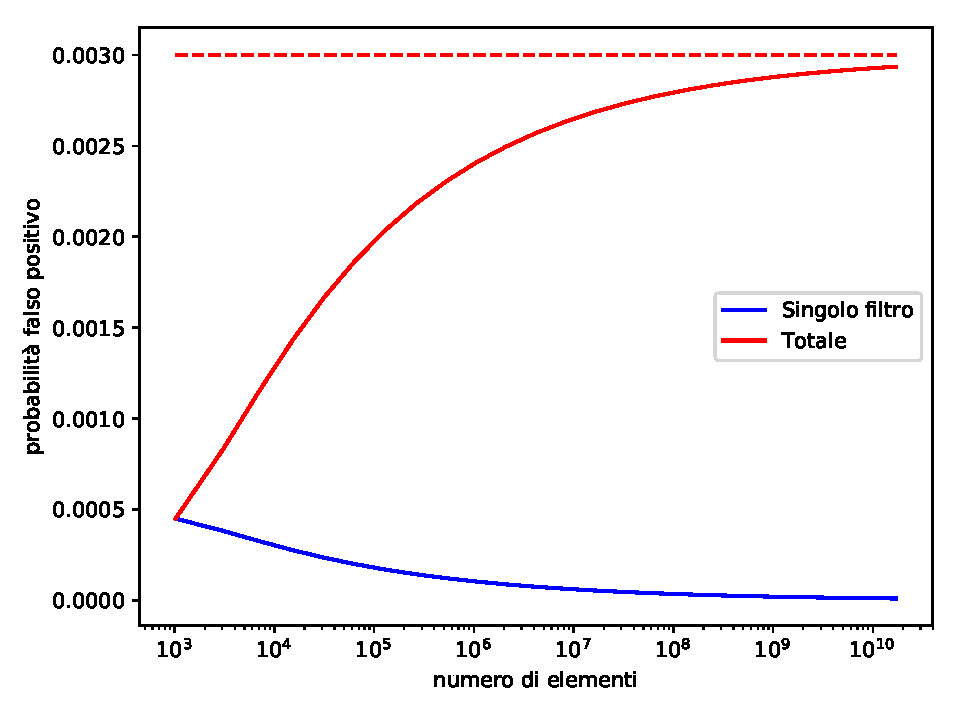
\includegraphics[width=\textwidth]{img/scalingbloom_error}
    }
  \end{minipage}
  \qquad
  \begin{minipage}[c]{0.7\textwidth}
    \subfloat[][Crescita delle funzioni di hash]{
      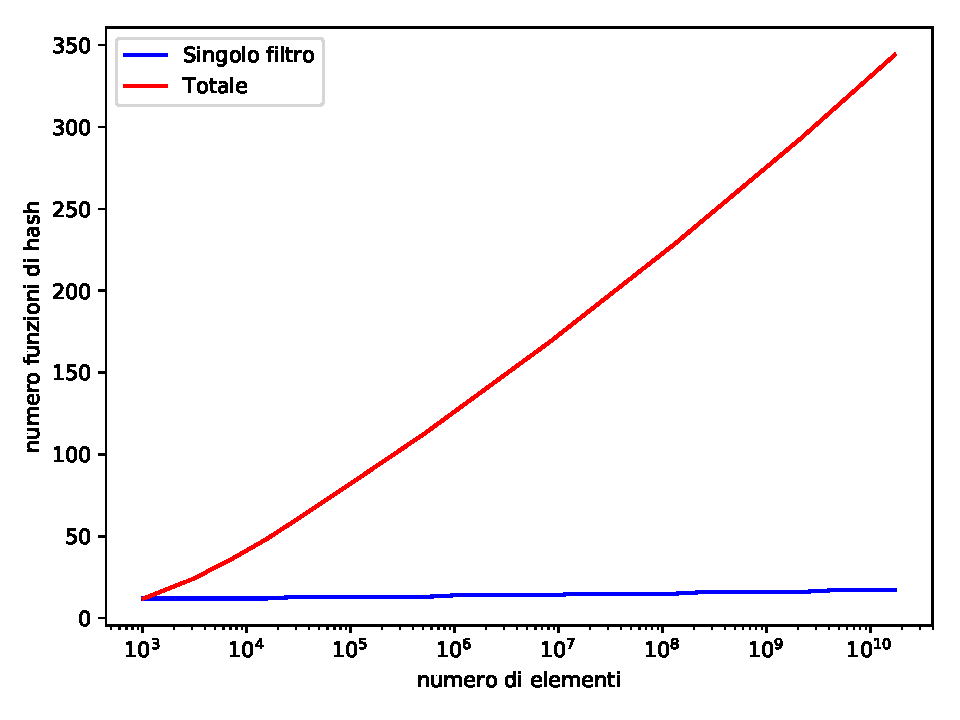
\includegraphics[width=\textwidth]{img/scalingbloom_hash}
    }
  \end{minipage}
  \qquad
  \begin{minipage}[c]{0.7\textwidth}
    \subfloat[][Crescita del consumo di memoria]{
      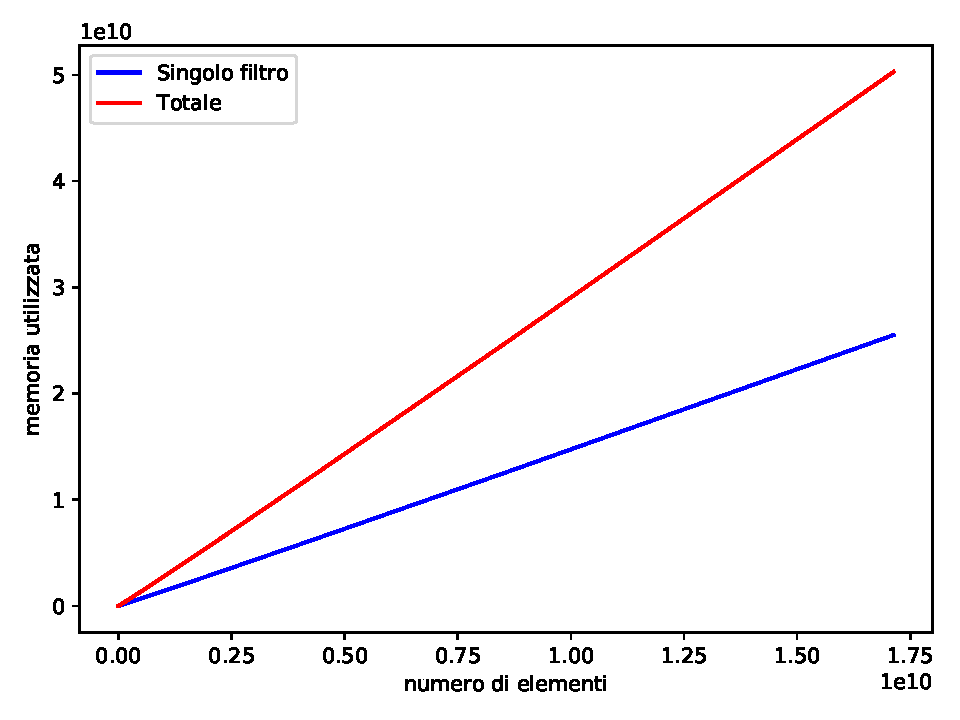
\includegraphics[width=\textwidth]{img/scalingbloom_memory}
    }
  \end{minipage}

  \caption{Andamento dei parametri del filtro scalabile in Redis in con\-fi\-gu\-ra\-zio\-ne di
  default}
  \label{fig:scalingbloom}
\end{figure}
















